\documentclass[12pt]{article}
\usepackage[utf8]{inputenc}
\usepackage[left=2.5cm, right=2.5cm, top=2.0cm]{geometry}
\usepackage{sectsty}
\usepackage{graphicx}
\usepackage{amsmath}
\usepackage{amssymb}
\usepackage{undertilde}
\usepackage{kbordermatrix}
\usepackage{listings}
\usepackage{ulem}
\usepackage{soul}
% \usepackage{tikz}
% \usepackage{pgfplots}
% \pgfplotsset{compat=1.16} 
\usepackage{siunitx}
\usepackage{pythonhighlight}
\usepackage{caption}
\usepackage{float}
\usepackage{url}
\usepackage{enumitem}
\usepackage{bm}
\usepackage{empheq}
\usepackage{tcolorbox}
\usepackage{framed}
\usepackage{xparse}
\usepackage{algorithm, algorithmic}
% \usepackage{algorithmic}
\usepackage{booktabs}
\usepackage{tabularx}
\usepackage{hyperref}


%  ---------------------- COMMANDS ---------------------------
% Double underline
\def\dunderline#1{\underline{\underline{#1}}}

% Shorten nonumber command
\def\nnb{\nonumber}

% Shorten boldsymbol command
\def\bs#1{\boldsymbol{#1}}

% Algorithmic newline
\def\algonewline{\STATE{ }}

% Eigenvectors of
\def\eigvecof{\text{eigenvectors of }}

% Eigenvalues of 
\def\eigvalof{\text{eigenvalues of }}

% Enclose in square brackets
\newcommand{\enclb}[1]{\left[#1\right]}
% Enclose in parenthesis
\newcommand{\enclp}[1]{\left(#1\right)}
% Enclose in curly brackets
\newcommand{\enclc}[1]{\left\{#1\right\}}

% Annotate first argument, text in second argument
\newcommand{\overtext}[2]{\overbrace{#1}^{\mathclap{\text{#2}}}}
\newcommand{\undertext}[2]{\underbrace{#1}_{\mathclap{\text{#2}}}}

% Normalization constant in multivariate normal
\newcommand{\mvnconst}[1]{\frac{1}{(2\pi)^{d/2} |#1|^{1/2}}}

% Exponential factor in multivariate normal
\newcommand{\mvnexpo}[3][x]{\exp \left[  -{\frac{1}{2}} (#1 - #2)^T #3^{-1} (#1 - #2) \right]}

% Multivariate normal
\newcommand{\mvn}[3][x]{\mvnconst{#3} \mvnexpo[#1]{#2}{#3}}

% For numbering in align* environment
\newcommand{\numberthis}{\addtocounter{equation}{1}\tag{\theequation}}

%  Sum notation w/ limits as argument and index as option
\newcommand{\sumlim}[3][i]{\sum\limits_{#1=#2}^{#3}}

%  Product notation w/ limits as argument and index as option
\newcommand{\prodlim}[3][i]{\prod\limits_{#1=#2}^{#3}}

%  Sum notation with only information beneath
\newcommand{\sumnolim}[1]{\sum\limits_{#1}}

%  Integral notation w/ limits as argument and index as option
\newcommand{\intlim}[2]{\int\limits_{#1}^{#2}}

%  Integral over whole domain notation, no args
\newcommand{\intinf}{\int\limits_{-\infty}^{\infty}}

%  Partial derivative notation, arg1: numerator, arg2: denominator
\newcommand{\pfrac}[3][ ]{\frac{\partial^{#1} #2}{\partial #3^{#1}}}

%  Derivative notation, arg1: numerator, arg2: denominator
\newcommand{\dvfrac}[3][ ]{\frac{\text{d}^{#1} #2}{\text{d} #3^{#1}}}

% When doing Gauss-Jordan, create arrow showing operations
\newcommand{\ro}[1]{\xrightarrow{\mathmakebox[\rowidth]{#1}}}

% ----------------------INVIRONMENTS---------------------------
% Item list with title
\newenvironment{titlemize}[1]{%
  \paragraph{#1}
  \begin{itemize}}
  {\end{itemize}}

  % Enum list with title
\newenvironment{titleenum}[1]{%
  \paragraph{#1}
  \begin{enumerate}}
  {\end{enumerate}}

  % Augmented matrix (matrix with vertical line)
\newenvironment{sysmatrix}[1]
  {\left(\begin{array}{@{}#1@{}}}
  {\end{array}\right)}

 % Make matrices with more spacing
\makeatletter
\renewcommand*\env@matrix[1][\arraystretch]{%
  \edef\arraystretch{#1}%
  \hskip -\arraycolsep
  \let\@ifnextchar\new@ifnextchar
  \array{*\c@MaxMatrixCols c}}
\makeatother

% \renewcommand*{\arraystretch}{1.5}

\newlength{\rowidth}% row operation width
\AtBeginDocument{\setlength{\rowidth}{3em}}

\floatname{algorithm}{Algorithm}
\renewcommand{\algorithmicrequire}{\textbf{Input:}}
\renewcommand{\algorithmicensure}{\textbf{Output:}}

\begin{document}
\title{\textbf{INF367A Exercise 5}}
\author{Naphat Amundsen}
\maketitle
\sectionfont{\fontsize{14}{15}\selectfont}
\subsectionfont{\fontsize{12}{15}\selectfont}
\subsubsectionfont{\fontsize{12}{15}\selectfont}
\graphicspath{ {./images/} }

\ifx
\begin{figure}[H]
	\centering
	\includegraphics[scale=0.8]{Figure_2}
	\caption{Insert caption here}
\end{figure}
\fi



\section{Introduction}
This exercise is about Bayesian inference on sample datasets. The functions are continuous, and we are supposed to utilize conjugate priors to estimate parameters. 

In case future self forgets: Normally, when you want to fit a probability density function to your data you find the MLEs for the model parameters. Now, we don't really care what the maximum likelihood actually is, as long as we maximize it. So when deriving MLEs you can basically remove every factor that does not depend on the parameter you want to optimize for since they are monotonic transformations (preserves extrema). This gives us much freedom when deriving. 

When doing stuff the Bayesian way, we actually include the prior into the equation. So instead of just maximizing likelihood, we maximize the likelihood times the prior: $P(X|\theta)P(\theta)$. In this exercise (and often generally) we assume that the parameter itself is distributed with some function. When simplifying $P(X|\theta)P(\theta)$ we can sometimes get the equation into a form that is proportional to a probability density function. If you do manage to get $P(X|\theta)P(\theta)$ in a form of another pdf, you have found a conjugate prior. You can then easily use Monte Carlo approximation to estimate the optimal parameter value since most known distributions are probably implemented by someone already. 

\section{Poisson-Gamma}
    \begin{tcolorbox}
        \begin{enumerate}
            \item \textbf{Poisson-Gamma}\\
            Poisson distribution can be used to model count data. Suppose you have $n$ i.i.d. observations $X = {\{x_i\}}_{i=1}^n$ from a $\Poisson{\lambda}$ distribution with a rate parameter $\lambda$ that has a conjugate prior $\lambda \sim \Gamma{a,b}$ with the shape and rate hyperparameters a and b.
            \begin{enumerate}
                \item Derive the posterior distribution $P(\lambda|x)$.
                \item Load the data set exercise5\_1.txt (100 one-dimensional data points). Compute the posterior of $\lambda$ given this data.
                \item Estimate the predictive distribution using Monte Carlo approximation. Plot the histogram of the predictive samples. Compare it to the original data. Do your results make sense? (If you are inclined to answer no then you have probably done something wrong along the way.)
                \item Compute 50\% and 95\% credible intervals for the predictive distribution. Hint: You should start by sorting your samples.
            \end{enumerate}
        \end{enumerate}
        Note: There are several different ways to parameterize the gamma distribution.
        If you use the gamma distribution from scipy, then Gamma(a0,b0) distribution
        is specified by gamma(a=a0, scale=1/b0).
    \end{tcolorbox}

    \def\Ppdf#1{\frac{\lambda^{#1} e^{-\lambda}}{{#1}!}}
    \def\Ppdfu#1{\lambda^{#1} e^{-\lambda}}
    \def\ld{\lambda}

    \textbf{Solution:}\\
    \textbf{1a)} Poisson distribution is:
    \begin{align}
        P(K=k) = \frac{\ld^k e^{-\ld}}{k!}
    \end{align}
    Then assuming that data points are i.i.d
    \begin{align}
        P(\ld | x) &= \frac{P(\ld) P(x|\ld)}{P(x)} \propto P(\ld) P(x | \ld) \\
        &= \frac{1}{\Gamma(a)}b^a \ld^{a-1} e^{-b\ld} \left[ \Ppdf{x_1} \cdot \Ppdf{x_2} \cdot \ldots \cdot \Ppdf{x_n} \right] \\
        &\propto \ld^{a-1} e^{-b\ld} \left( \Ppdfu{x_1} \cdot \Ppdfu{x_2} \cdot \ldots \cdot \Ppdfu{x_n} \right) \\
        &= \ld^{a-1 + \sumlim{1}{n} x_i} e^{-(n+b)\ld} \\
        &\dunderline{\propto \operatorname{Gamma}(a - 1 + \sumlim{1}{n} x_i, n+b)}
    \end{align}

    \textbf{1b)} The prior distribution for $\lambda$ is plotted against the posterior distribution. The prior is $\Gammaf{2,2}.$
    \begin{figure}[H]
        \centering
        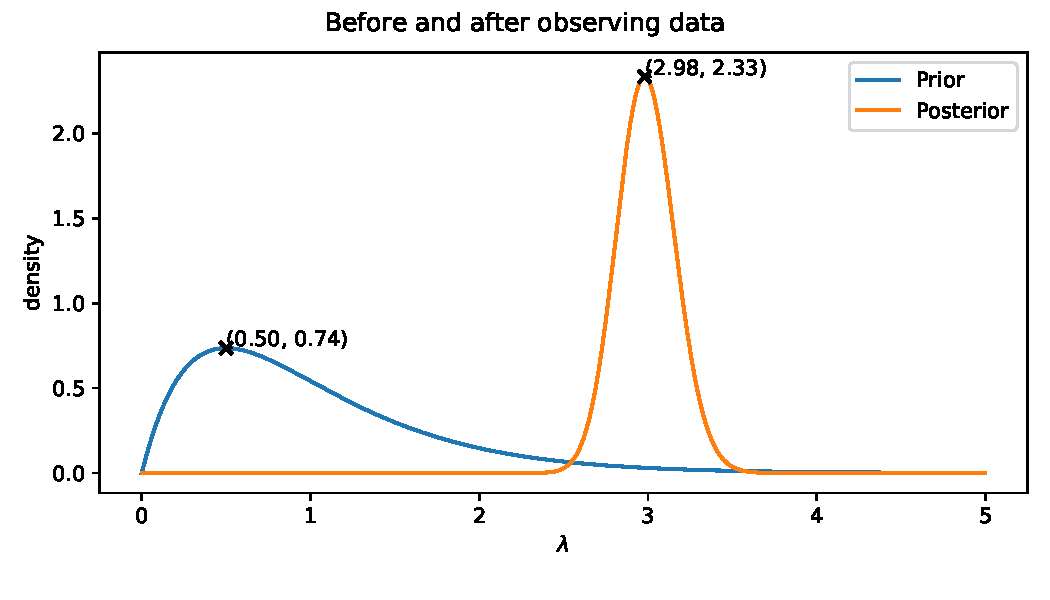
\includegraphics[width=0.9\textwidth]{1b.pdf}
        \caption{We can see that the posterior distribution centers around $\lambda \approx 3$}
    \end{figure}

    \textbf{1c)} Then using the posterior approximated $\lambda$, we try to sample from the predictive function $(\Poisson{\lambda})$ to see if the distribution looks alike. 
    \begin{figure}[H]
        \centering
        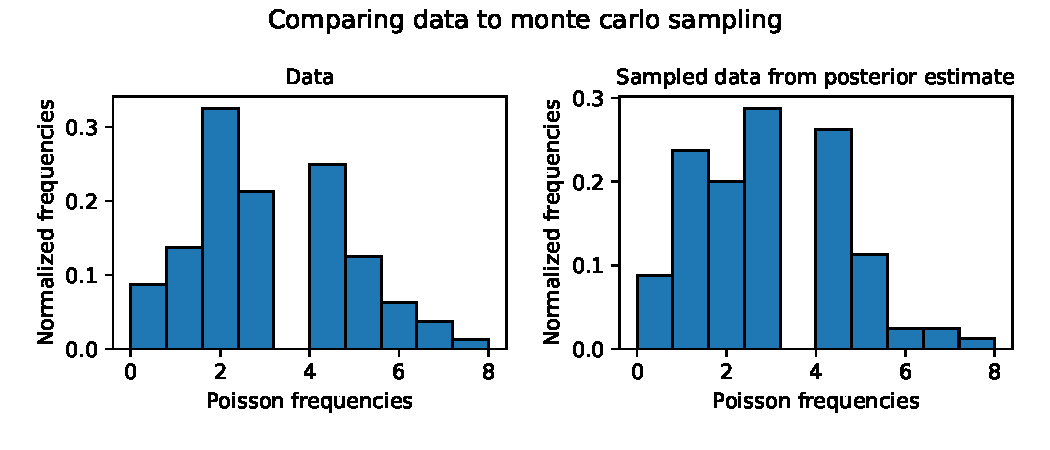
\includegraphics[width=0.9\textwidth]{1c.pdf}
        \caption{The data and the monte carlo sampled points seem to come from the same distributions.}
    \end{figure}

    \textbf{1d)} \\  
    \indent 50\% Credibility interval: (1, 3) \\
    \indent 95\% Credibility interval: (0, 6)

\section{Multivariate Gaussian}
    \begin{tcolorbox}
        \begin{enumerate}[start=2]
            \item \textbf{Multivariate Gaussian}\\
            Suppose we have $N$ i.i.d observations $X = {x_i}_{i=1}^N$ from a multivariate Gaussian distribution 
            $$ \bs x_i | \bs \mu \sim \mathcal{N}(\bs \mu, \bs \Sigma)$$

            with unknown mean parameter $\mu$ and a known covariance matrix $\Sigma$. As prior information on the mean parameter we have
            $$\bs \mu \sim \mathcal{N}(\bs m_0, \bs S_0).$$
            
            \begin{enumerate}
                \item Derive the posterior distribution $P(\mu|X)$ of the mean parameter $\mu$. Hints: It may be more comfortable to work with the log-posterior $\log P(\mu|X)$. You can drop all terms that do not depend on $\mu$. The log-posterior of a multivariate Gaussian is a second degree polynomial so you can use “completing the square”.
                \item Load the data set exercise5\_2.txt(100 two-dimensional data points). Compute the posterior of $\mu$ given this data. Compute the posterior of $\mu$ given this data.
                \item (Optional) Plot the posterior in 3D. Do your results make sense?
            \end{enumerate}
        \end{enumerate}
    \end{tcolorbox}

    \textbf{2a)} Multivariate normal distribution probably density function:
    \begin{align}
        f_N(x_i | \mu, \Sigma) = \mvn[x]{\mu}{\Sigma} 
    \end{align}
    Then to calculate the posterior:
    \begin{align}
        P(\mu | X) &= \frac{P(\mu) P(X|\mu)}{P(X)} \propto P(\mu) P(X | \mu) \\
        &= \mvnexpo[\mu]{m_0}{S_0} \prodlim[i]{1}{N} \mvnexpo[x_i]{\mu}{\Sigma} \\ 
    \end{align}

    Solve for the logarithm of the posterior instead in order to make math easier. The goal here is to get the terms in quadratic form:
    \begin{align}
        \frac{1}{2} \theta^T A \theta + b^T \theta
    \end{align}
    which will implies that you have a Gaussian conjugate (if can get the quadratic form).

    \newcommand{\sn}{S_0^{-1}}
    \newcommand{\precmat}{\Sigma^{-1}}

    \begin{align}
        \log P(\mu | X) &= \log \mvnexpo[\mu]{m_0}{S_0} \\
        &+ \log \prodlim[i]{1}{N} \mvnexpo[x_i]{\mu}{\Sigma} \\
        &= -\frac{1}{2}(\mu-m_0)^T \sn (\mu-m_0) + \sumlim{1}{N} \log \mvnexpo[x_i]{\mu}{\Sigma} \\
        &= -\frac{1}{2}(\mu-m_0)^T \sn (\mu-m_0) + \sumlim{1}{N} -\frac{1}{2} (x_i-\mu)^T \Sigma^{-1} (x_i-\mu) \\
        &= -\frac{1}{2} \left[ (\mu-m_0)^T \sn (\mu-m_0) + \sumlim{1}{N} (x_i-\mu)^T \Sigma^{-1} (x_i-\mu) \right] \\
        &= -\frac{1}{2} \big[ \mu^T\sn\mu - m_0^T\sn\mu - \mu^T\sn m_0 - m_0^T \sn m_0 \\
        &+ \sumlim{1}{N} x_i^T \precmat x_i - x_i^T \precmat \mu - \mu^T \precmat x_i + \mu^T \precmat \mu\big] \\
        &\propto -\frac{1}{2} \big[ \mu^T\sn\mu - m_0^T\sn\mu - \mu^T\sn m_0 \\
        &+ \sumlim{1}{N} - x_i^T \precmat \mu - \mu^T \precmat x_i + \mu^T \precmat \mu \big] \\ 
    \end{align}
    When we have a symmetric $A$, then this relation holds: $x^T A y = y^T A x$
    \begin{align}
        \Rightarrow \log P(\mu | X) &\propto -\frac{1}{2} \big[ \mu^T\sn\mu - m_0^T\sn\mu - \mu^T\sn m_0 \\
        &+ \sumlim{1}{N} - x_i^T \precmat \mu - \mu^T \precmat x_i + \mu^T \precmat \mu \big] \\ 
        &= -\frac{1}{2} \big[ \mu^T\sn\mu - m_0^T\sn\mu - m_0^T\sn \mu \\
        &+ \sumlim{1}{N} - x_i^T \precmat \mu - x_i^T \precmat \mu + \mu^T \precmat \mu \big] \\ 
        &= -\frac{1}{2} \big[ \mu^T\sn\mu - 2 m_0^T\sn\mu + \sumlim{1}{N} - 2 x_i^T \precmat \mu + \mu^T \precmat \mu \big] \\
        &= -\frac{1}{2} \big[ \mu^T\sn\mu - 2 m_0^T\sn\mu - N \mu^T \precmat \mu - 2\sumlim{1}{N} x_i^T \precmat \mu \big] \\
        &= -\frac{1}{2} \big[ \mu^T\sn\mu + N \mu^T \precmat \mu - 2 N \bar{X}^T \precmat \mu - 2 m_0^T\sn\mu  \big] \\
        &= -\frac{1}{2} \left[ \mu^T\left(\sn+N\precmat\right)\mu  - 2\left(N\bar{X}^T\precmat + m_0^T\sn\right)\mu \right] \\
        &= -\frac{1}{2} \mu^T\left(N\precmat+\sn\right)\mu  + \left(N\bar{X}^T\precmat + m_0^T\sn\right)\mu 
    \end{align}

    We have now obtained quadratic form. Let
    \begin{align}
        A = \left(N\precmat+\sn\right), b^T = \left(N\bar{X}^T\precmat + m_0^T\sn\right)
    \end{align}
    Then by completing the square, we can obtain the parameters $\mu_N, \Sigma_N$ for a Gaussian (see lecture slides)
    \begin{align}
        \Sigma_N &= A^{-1} = \left(N\precmat+\sn\right)^{-1} \\
        \mu_N &= A^{-1}b = \left(N\precmat+\sn\right)^{-1} \left(N\precmat\bar{X} + \sn m_0\right)\\
        &\dunderline{\Rightarrow P(\mu| X) = N(\mu|\mu_N, \Sigma_N)}
    \end{align}

    \textbf{2b,c)} Doing another monte carlo sampling, we can compare the prior and posterior distributions for $\mu$. 
    \begin{figure}[H]
        \centering
        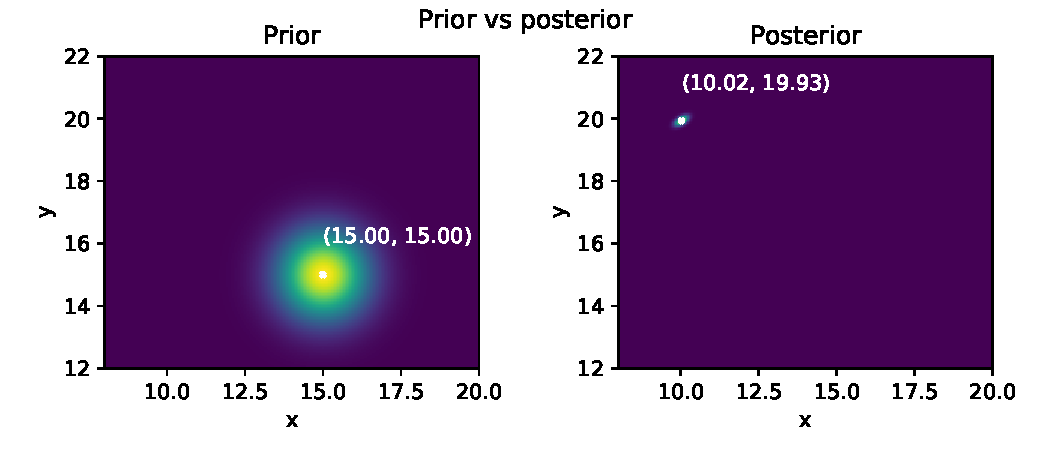
\includegraphics[width=0.9\textwidth]{2c.pdf}
        \caption{Heatmaps representing the densities on the $\mathbb{R}^2$ input space. The prior has variance 1 and is centered at (15,15). The posterior shrunk in size and huddled around $\approx (10,20)$. The real $\mu$ is probably $(10,20)$ since they are so nice numbers.} 
    \end{figure}

% \bibliographystyle{apalike}
% \bibliographystyle{ieeetran}
% \bibliography{citations}

\appendix
\section{Task 1 Code}
\inputpython{ex1_code.py}{0}{1000}
\section{Task 2 Code}
\inputpython{ex2_code.py}{0}{1000}

\end{document}

